%% Chapter 4: The Recursive CoMO Model

\chapter{The Recursive CoMO Model}
\label{chap:model}
In Chapter~\ref{chap:abm} we showed that under network effects, standard research methods give biased estimates of the causal effect of SMU on WB\@. This chapter introduces a model specification dealing with this issue by explicitly modelling the CoMO mechanism and the network structure. We present the model structure and equations, illustrate them with an example, and establish identification. This lays the theoretical framework for the estimation strategies we will employ in Chapter~\ref{chap:estimation}, where we develop both 2SLS and ML estimators.

When showing identification, we follow two paths, corresponding to the two estimators later developed. The first is to adapt the reasoning of \textcite{Bramoulle2009}, exploiting network structure for identification. This corresponds to the assumptions made for the 2SLS estimator. The second is to exploit the covariance structure of the model, due to the Gaussian likelihood, requiring the normality assumption underpinning the ML estimator. The identification results of this chapter (Propositions~\ref{prop:screen_identification},~\ref{prop:wb_identification}, and~\ref{prop:wb_ml_identification}) thus rely on existing tools, but are our own original derivations for the recursive CoMO model.

The modelling framework of this chapter addresses the central finding from Chapter~\ref{chap:abm} that network effects lead to bias. However, it does so on a static DGP, which makes identification and estimation tractable at a cost to realism. We discuss this simplification cost in Section~\ref{sec:model:discussion} and Section~\ref{sec:discussion_conclusion:gap}.

%% Section 4.1: Model Components
\section{Model Components}
\label{sec:model:components}
To make a model taking network structure into account, we first need a framework for modelling the relationship between SMU and WB\@. We do this by providing an equation for each, with a \emph{recursive} structure connecting them together, meaning that we let SMU influence WB, but not the other way around. The model also needs to take into account a network of $n$ individuals, with connections among the individuals. As we will see, we do this by a row-normalised adjacency matrix $\mat{G}$ (see Definition~\ref{def:row_normalised} and Section~\ref{sec:bg:networks} for theory on the adjacency matrix).

For the modelling of SMU and WB itself, we let each individual $i$ have the following variables:
\begin{itemize}
    \item Observed social media use $s_i$
    \item Observed well-being $y_i$
\end{itemize}

As in Chapter~\ref{chap:abm}, we let observed SMU be measured in hours per day, and observed WB be a continuous scale from $0$ to $10$. Each individual also has a set of neighbours (friends) $N_i \subseteq \{1, \ldots, n\}$, with these connections being represented in the adjacency matrix $\mat{G}$.

The model itself has a recursive structure, and consists of two equations modelling individuals' SMU and WB:
\begin{enumerate}
    \item \textbf{SMU equation}: An individual's SMU depends on peer SMU and exogenous factors.
    \item \textbf{WB equation}: An individual's WB depends on the individual's own SMU, the CoMO variable, peer WB, and exogenous factors.
\end{enumerate}

The recursive structure is advantageous as it allows the two equations to be estimated separately. Since SMU does not depend on WB, we can estimate the SMU equation based on only the observed $(\vect{s}, \mat{G})$. Similarly, the WB equation can be estimated from observed $(\vect{y}, \vect{s}, \mat{G})$ as it does not require any output from the SMU estimation.

%% Section 4.2: SMU Equation
\section{SMU Equation}
\label{sec:model:screen}
\subsection{Model Specification}

For the SMU equation we want to allow individual SMU to be realistic by including a baseline around which individuals vary, along with noise. We also want to include network effects, and do this through a term for the influence of the mean SMU of neighbours.

These components build the following model for the SMU of individual $i$:
\begin{equation}
\label{eq:screen_time}
    s_i = \beta_0 + \beta_1 \sbar_i + u_i, \quad i = 1, \ldots, n
\end{equation}

Here,

\begin{itemize}
    \item $\beta_0$ is a coefficient for baseline SMU
    \item $\beta_1$ is a coefficient that captures the peer influence on SMU $\sbar_i$, where $\sbar_i = \frac{1}{|N_i|}\sum_{j \in N_i} s_j = (\mat{G}\vect{s})_i$ is the average over the SMU of the peers of individual $i$ (defined through $\mat{G}$)
    \item $u_i \iid \N(0, \sigma_u^2)$ are independent normal error terms
\end{itemize}

For our purposes, it is also useful to have the equation in matrix form, as we will primarily use this later for parameter estimation. With $\vect{1} = (1, \ldots, 1)^\top$ denoting the vector of $n$ ones, $\vect{s} = (s_1, \ldots, s_n)^\top$ the vector of SMU values, and $\vect{u} = (u_1, \ldots, u_n)^\top$ the vector of errors, we can write the equation in matrix form as:

\begin{equation}
\label{eq:screen_matrix}
    \vect{s} = \beta_0 \vect{1} + \beta_1 \mat{G}\vect{s} + \vect{u}
\end{equation}

The focus point of this model is the $\beta_1$ parameter, which introduces the network effects. The parameter captures the degree of conformity to peers when it comes to SMU\@. When $\beta_1 > 0$, it draws the SMU of each individual towards the average of their peers. If $\beta_1 < 0$, individuals are non-conformist, and move in the opposite direction of their peer average. If $\beta_1 = 0$, the model does not include any influence from peers on individuals' SMU\@. Thus, this model can capture peer dynamics affecting individual SMU\@.

\subsection{Reduced Form with Distribution}

In preparation for estimation in Chapter~\ref{chap:estimation}, we follow the methods of \textcite[Sec.~2.3]{Bramoulle2009} and write the matrix version of the SMU equation in reduced form.

First, we rearrange terms in~\eqref{eq:screen_matrix}:

\begin{equation}
    \label{eq:screen_rearranged}
    (\mat{I} - \beta_1\mat{G})\vect{s} = \beta_0\vect{1} + \vect{u}
\end{equation}

We then make the following assumption:

\begin{assumption}[SMU Stability]
    \label{ass:screen_stability}
    The peer effect parameter satisfies $|\beta_1| < 1$.
\end{assumption}

Using Assumption~\ref{ass:screen_stability}, it follows from Proposition~\ref{prop:invertibility} in Section~\ref{sec:bg:sar} that $(\mat{I} - \beta_1\mat{G})$ is invertible, and we can thus write our reduced form of the equation:
\begin{equation}
\label{eq:screen_reduced}
    \vect{s} = (\mat{I} - \beta_1\mat{G})^{-1}\beta_0\vect{1}
             + (\mat{I} - \beta_1\mat{G})^{-1}\vect{u}
\end{equation}

We note that $\vect{u} \sim \N(\vect{0}, \sigma_u^2\mat{I})$ is the only random term in the reduced form equation~\eqref{eq:screen_reduced}, and so we can immediately write down the distribution of $\vect{s}$:

\begin{equation}
    \label{eq:s_distribution}
    \vect{s} \sim \N\left((\mat{I} - \beta_1\mat{G})^{-1}\beta_0\vect{1}, \;
    \sigma_u^2(\mat{I} - \beta_1\mat{G})^{-1}
    [(\mat{I} - \beta_1\mat{G})^{-1}]^\top\right)
\end{equation}

This follows from the following property of linear transformations of multivariate normal vectors: If $\vect{u} \sim \N(\vect{\mu}, \mat{\Sigma})$, then $\mat{A}\vect{u} + \vect{b} \sim \N(\mat{A}\vect{\mu} + \vect{b}, \mat{A}\mat{\Sigma}\mat{A}^\top)$, applied to $\N(\vect{\mu}, \mat{\Sigma}) = \N(\vect{0}, \sigma_u^2\mat{I})$.

%% Section 4.3: WB Equation
\section{WB Equation}
\label{sec:model:wellbeing}
\subsection{The CoMO Term}
\label{sec:model:como}
The introduction of our asymmetric, network-structured CoMO specification is a novel way of capturing peer effects within a structural network model. In Chapter~\ref{chap:abm} we showed how ignoring network effects of social comparison leads to bias in estimation of the effect of SMU on WB\@. The CoMO mechanism, introduced in the SMU--WB context by \textcite[Eqs.~1--2]{DahlFoldnesGronneberg2024} and motivated in Section~\ref{sec:bg:social_comparison}, captures the cost of missing out on shared context and experiences that individuals incur when their SMU is less than that of their peers. Thus, we are able to capture network effects in our model that would otherwise lead to biased estimates.

We define CoMO in our model as follows.

\begin{definition}[Cost of Missing Out]
    \label{def:como}
    The CoMO term for individual $i$ is:
    \begin{equation}
        c_i = \max(0, \sbar_i - s_i) = (\sbar_i - s_i)^+
    \end{equation}
\end{definition}

Here, $\sbar_i$ is the average SMU of the peers of individual $i$, as defined in Equation~\eqref{eq:screen_time}. In Figure~\ref{fig:como_function} we provide a graphical illustration of the CoMO effect.

\begin{figure}[htbp]
    \centering
    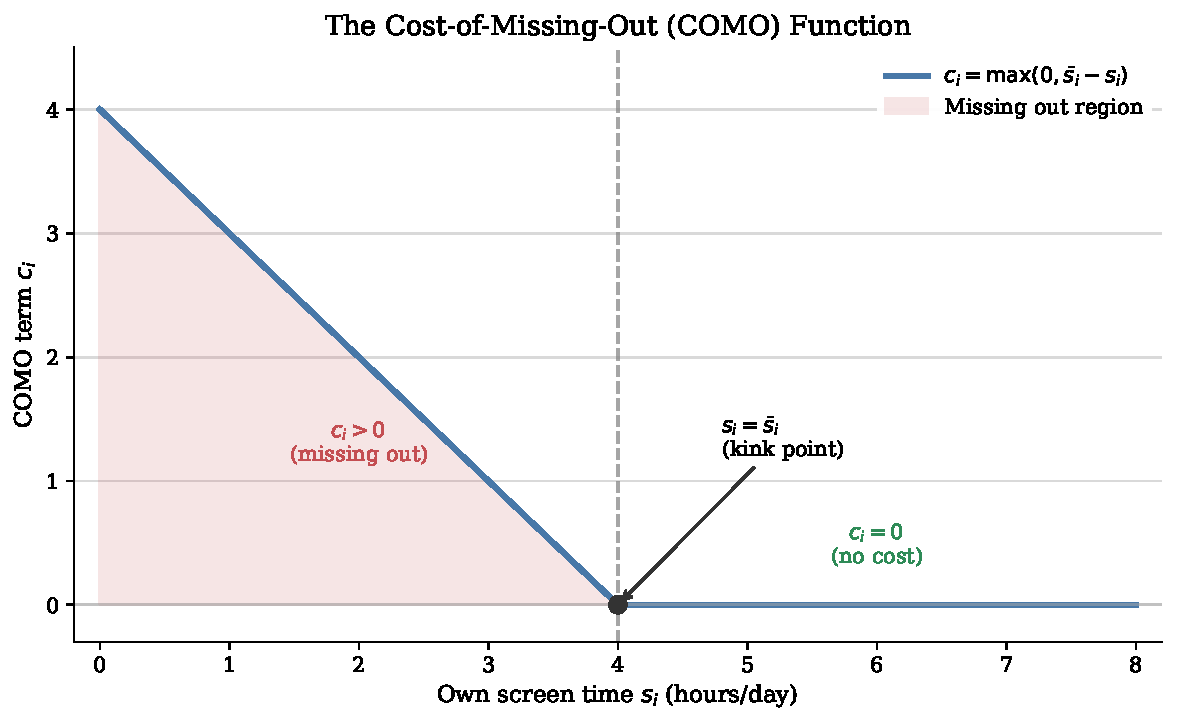
\includegraphics[width=0.8\textwidth]{figures/como_function.pdf}
    \caption[The CoMO function $c_i = \max(0, \sbar_i - s_i)$]{The blue line shows the CoMO function $c_i = \max(0, \sbar_i - s_i)$ for an individual with peer average $\sbar_i = 4$. When $s_i$ falls below the peer average $\sbar_i$, we get a positive CoMO term. When $s_i = \sbar_i$, we get a kink, showing the asymmetry of the CoMO mechanism.}
    \label{fig:como_function}
\end{figure}

The non-linear form of the CoMO term comes from our belief that individuals might pay a cost for having SMU below their peers, but that having SMU above the peer level does not necessarily give a direct positive effect on WB\@. Hence, we use the max operator, which leads to a mechanism that kicks in when $s_i < \sbar_i$. When an individual uses social media less than their peers, they experience the cost of missing out in proportion to the difference. When $s_i \geq \sbar_i$, i.e., when an individual uses social media at least as much as peers, there is no CoMO effect, $c_i = 0$. When the coefficient on CoMO in the WB equation is negative, CoMO reduces WB\@.

We also write the CoMO mechanism in vector notation:
\begin{equation}
    \vect{c} = (\mat{G}\vect{s} - \vect{s})^+ = \max(\vect{0}, \mat{G}\vect{s} - \vect{s})
\end{equation}
Here, the max is applied element-wise.

\subsection{Model Specification}

The WB part of the model is more complicated than the SMU part, as this is where we introduce the CoMO mechanism defined above. We want to let the network effects of neighbour SMU and WB influence the WB of each individual, as well as include a realistic baseline with random variation.

To include all these aspects, we use the following equation to model the WB of individual $i$:

\begin{equation}
\label{eq:wellbeing}
    y_i = \gamma_0 + \gamma_1 s_i + \gamma_2 c_i + \gamma_3 \ybar_i
        + \varepsilon_i, \quad i = 1, \ldots, n
\end{equation}

Here,

\begin{itemize}
    \item $\gamma_0$ is a coefficient for baseline WB
    \item $\gamma_1$ is a coefficient for the direct effect of individual SMU on WB
    \item $\gamma_2$ is a coefficient that captures the effect of the CoMO term $c_i$ on WB (Definition~\ref{def:como})
    \item $\gamma_3$ is a coefficient that captures the influence of peer WB, $\ybar_i$, on individual WB, where $\ybar_i = \frac{1}{|N_i|}\sum_{j \in N_i} y_j = (\mat{G}\vect{y})_i$ is the average WB of the peers of individual $i$ (defined through $\mat{G}$)
    \item $\varepsilon_i \iid \N(0, \sigma_\varepsilon^2)$ are independent normal error terms
\end{itemize}

A result of this specification is that the marginal effect of own SMU on WB is piecewise. This comes from the CoMO formulation $c_i = \max(0, \sbar_i - s_i)$. When holding the peer average $\sbar_i$ fixed, $\partial y_i / \partial s_i = \gamma_1 - \gamma_2$ when $s_i < \sbar_i$, and $\partial y_i / \partial s_i = \gamma_1$ when $s_i \geq \sbar_i$.

The $\gamma_1$, $\gamma_2$, and $\gamma_3$ parameters of the specification are the most interesting, and we provide a short interpretation of them here. $\gamma_1$ captures the direct effect of an individual's own SMU on their WB\@. Thus, if $\gamma_1 < 0$, a high SMU leads to lower WB, while $\gamma_1 > 0$ implies the opposite. For $\gamma_2$ we similarly have that the parameter controls the influence of the CoMO effect on individual WB\@. If $\gamma_2 < 0$, the CoMO effect has a negative influence on the WB of individuals who have less SMU than their peers. If $\gamma_2 = 0$, there is no social comparison, and when $\gamma_2 > 0$, this would imply a positive effect of lower SMU coming from peer comparison. Lastly, $\gamma_3$ controls the influence of peer WB on own WB\@. If $\gamma_3 > 0$, the positive WB of peers has a positive influence, while $\gamma_3 < 0$ would encode a cost of being around peers with high WB\@.

As with the SMU equation, we want a version in matrix form. Using the same notation as before, we introduce the design matrix
\begin{equation}
    \mat{X} = [\vect{1}, \vect{s}, \vect{c}]
\end{equation}
and let $\gammavec = (\gamma_0, \gamma_1, \gamma_2)^\top$ denote the parameter vector corresponding to the columns of $\mat{X}$. The matrix form of the WB equation is then:

\begin{equation}
    \label{eq:wellbeing_matrix}
    \vect{y} = \mat{X}\gammavec + \gamma_3\mat{G}\vect{y} + \vect{\varepsilon}
\end{equation}

\subsection{Reduced Form with Distribution}
For the purpose of model estimation in Chapter~\ref{chap:estimation}, we also write the WB equation in reduced form.

We first let $\Ay = \mat{I} - \gamma_3\mat{G}$. Then, rearranging Equation~\eqref{eq:wellbeing_matrix}, we get:

\begin{equation}
    \Ay\vect{y} = \mat{X}\gammavec + \vect{\varepsilon}
\end{equation}

We then make the following assumption:

\begin{assumption}[WB Stability]
    \label{ass:wb_stability}
    The peer effect parameter satisfies $|\gamma_3| < 1$.
\end{assumption}

Under Assumption~\ref{ass:wb_stability} it follows from Proposition~\ref{prop:invertibility} in Section~\ref{sec:bg:sar} that $\Ay$ is invertible, and we can thus write our reduced form of the equation:

\begin{equation}
    \label{eq:wellbeing_reduced}
    \vect{y} = \Ay^{-1}\mat{X}\gammavec + \Ay^{-1}\vect{\varepsilon}
\end{equation}

For the distribution of $\vect{y}$, the WB equation is more difficult to work with than the SMU equation. This is because the reduced form~\eqref{eq:wellbeing_reduced} includes $\vect{s}$ in two separate places in $\mat{X} = [\vect{1}, \vect{s}, \vect{c}]$: both through the direct effect of $\vect{s}$, and through $\vect{s}$ being part of the CoMO term $\vect{c} = \max(\vect{0}, \mat{G}\vect{s} - \vect{s})$. As the CoMO term is a non-linear function of $\vect{s}$ we do not get a straightforward unconditional distribution of $\vect{y}$.

However, if we condition on $\vect{s}$, both $\vect{s}$ and $\vect{c}$ will be fixed, and there only remains one random component: $\vect{\varepsilon} \sim \N(\vect{0}, \sigma_\varepsilon^2\mat{I})$. Thus, for the conditional case, we can apply the same linear transformation property as for the distribution of $\vect{s}$. Doing this, we get the following conditional distribution:

\begin{equation}
\label{eq:wellbeing_conditional_dist}
    \vect{y} \mid \vect{s} \sim \N\!\left(\Ay^{-1}\mat{X}\gammavec, \;\;
    \sigma_\varepsilon^2 \Ay^{-1}[\Ay^{-1}]^\top\right)
\end{equation}

The fact that we can get this conditional distribution comes from the recursive structure of our model. This distribution will be central when we develop an estimation strategy based on ML in Chapter~\ref{chap:estimation}. Since $\vect{s}$ is observed, we can condition on it directly and work with the multivariate normal likelihood of~\eqref{eq:wellbeing_conditional_dist}, avoiding the trouble caused by the non-linearity of the CoMO term.

%% Section 4.4: Illustrative Example
\section{Illustrative Example}
\label{sec:model:example}
Before moving to model assumptions and identification, we illustrate the various components of our model by working through an example with $n = 4$ individuals. The example also previews the network-lag intuition that underlies the identification argument in Section~\ref{sec:model:identification}.

\subsection{Network Structure}

To define the network structure, we need to decide what connections to make between the four individuals. We define the following relationships: individual 1 is friends with 2 and 3, individual 2 is friends with 1 and 4, individual 3 is friends with 1 only, and individual 4 is friends with 2 only. This creates an intransitive network, as 3 and 4 are not directly connected, but are still connected through other individuals. This feature of intransitivity will be used in Section~\ref{sec:model:identification}.

Based on these connections, the row-normalised adjacency matrix is:
\begin{equation}
    \mat{G} = \begin{pmatrix}
        0 & 1/2 & 1/2 & 0 \\
        1/2 & 0 & 0 & 1/2 \\
        1 & 0 & 0 & 0 \\
        0 & 1 & 0 & 0
    \end{pmatrix}
\end{equation}

In Figure~\ref{fig:network_example} we visualise this network along with the computed values below.

\begin{figure}[htbp]
    \centering
    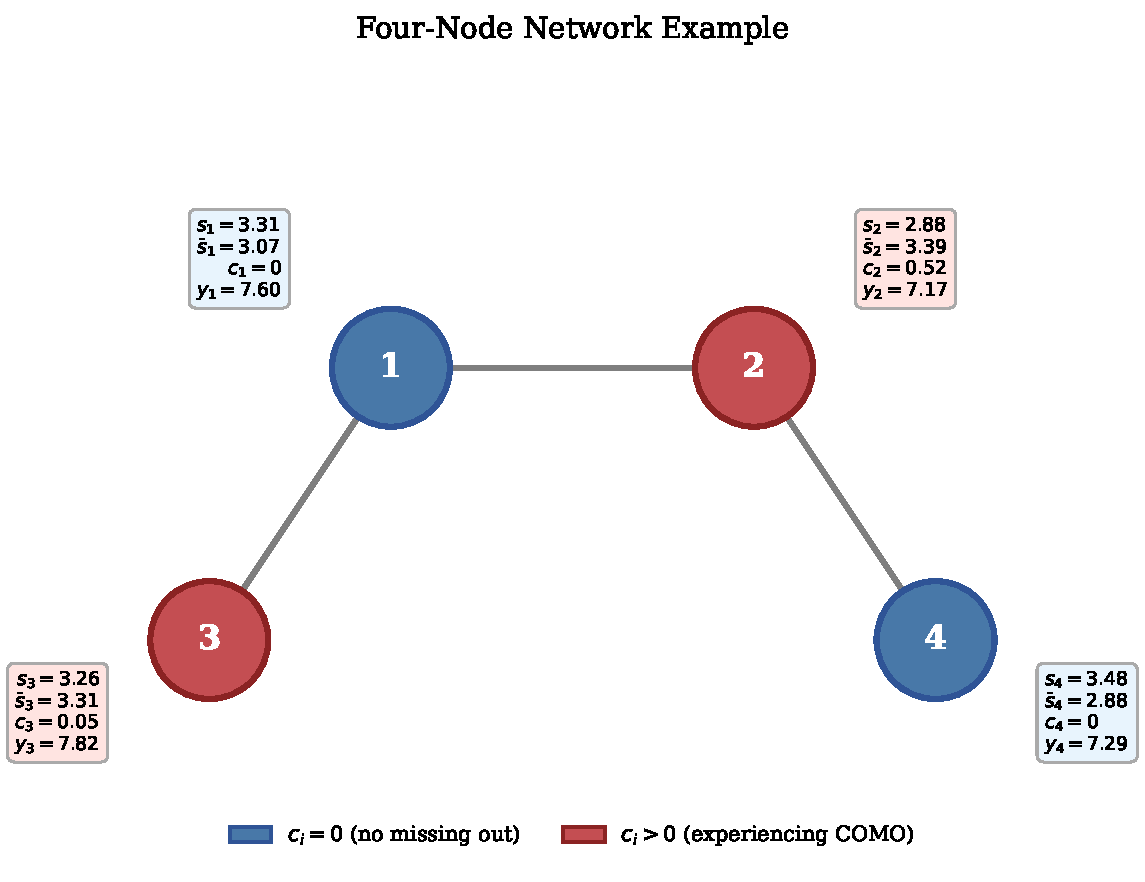
\includegraphics[width=0.85\textwidth]{figures/network_example_chapter_4.pdf}
    \caption[Four-node network example with SMU, peer average, CoMO, and WB]{Illustration of the four-node network used in the example. Nodes represent individuals, and edges represent network connections. For each node we show the values of individual SMU, $s_i$, the peer average $\sbar_i$, the CoMO term $c_i$, and the WB $y_i$. Individual 2 (red) experiences the largest CoMO effect, as they have SMU notably below their peer average.}
    \label{fig:network_example}
\end{figure}

\subsection{Computation of SMU, CoMO, and WB}

We suppose that the true parameters are $\beta_0 = 2.5$, $\beta_1 = 0.2$, $\sigma_u = 0.5$ ($\sigma_u^2 = 0.25$). This represents a baseline of 2.5 hours of daily SMU, a positive association with average peer use, and moderate variation. We also suppose that the errors are given as $\vect{u} = (0.2, -0.3, 0.1, 0.4)^\top$.

Using the reduced form $\vect{s} = (\mat{I} - \beta_1\mat{G})^{-1}(\beta_0\vect{1} + \vect{u})$ we can then calculate $\vect{s}$, and get (after matrix inversion):

\begin{equation}
    \vect{s} \approx (3.31, 2.88, 3.26, 3.48)^\top
\end{equation}

Using $\mat{G}$ we can then also calculate the peer averages of each individual:

\begin{equation}
    \mat{G}\vect{s} \approx (3.07, 3.39, 3.31, 2.88)^\top
\end{equation}

We use the peer averages to calculate the CoMO experienced by each individual:

\begin{align}
    c_1 &= \max(0, 3.07 - 3.31) = 0 \\
    c_2 &= \max(0, 3.39 - 2.88) = 0.52 \\
    c_3 &= \max(0, 3.31 - 3.26) = 0.05 \\
    c_4 &= \max(0, 2.88 - 3.48) = 0
\end{align}

In this example, individual 2 experiences the largest CoMO effect, as they use social media notably less than their peer average. Individual 3 experiences a negligible CoMO ($c_3 = 0.05$), while individuals 1 and 4 have $c_i = 0$.

Now, we suppose that the true parameters of the WB equation are $\gamma_0 = 7$, $\gamma_1 = -0.3$, $\gamma_2 = -0.5$, $\gamma_3 = 0.2$, and $\sigma_\varepsilon = 0.4$ ($\sigma_\varepsilon^2 = 0.16$), with observed variation $\vect{\varepsilon} = (0.1, -0.2, 0.3, -0.1)^\top$ for the individuals. This represents a high baseline WB of 7, with a negative effect of SMU and CoMO, a slightly positive effect of peer WB, and moderate variation.

These parameters give the following WB equation:

\begin{equation}
    y_i = 7 - 0.3 s_i - 0.5 c_i + 0.2 \ybar_i + \varepsilon_i
\end{equation}

Inserting our values in the reduced form of Equation~\eqref{eq:wellbeing_reduced} yields:

\begin{equation}
    \vect{y} \approx (7.60, 7.17, 7.82, 7.29)^\top
\end{equation}

We note that individual 2 has the lowest WB, partly caused by the CoMO term ($c_2 = 0.52$), which contributes $-0.5 \times 0.52 = -0.26$ to their WB\@.

\subsection{Network Lags and Friends-of-Friends}
\label{sec:model:network_lags}
A feature of the network that will become useful in Section~\ref{sec:model:identification} is that powers of $\mat{G}$ encode indirect network connections. Continuing our example above, we illustrate by computing $\mat{G}^2$:

\begin{equation}
    \mat{G}^2 = \begin{pmatrix}
        3/4 & 0 & 0 & 1/4 \\
        0 & 3/4 & 1/4 & 0 \\
        0 & 1/2 & 1/2 & 0 \\
        1/2 & 0 & 0 & 1/2
    \end{pmatrix}
\end{equation}

Even though $G_{14} = 0$, we have $(\mat{G}^2)_{14} = 1/4 > 0$. Thus, although individuals 1 and 4 are not directly connected, they are linked in $\mat{G}^2$ through their shared friend 2. A change in individual 4's SMU can only reach individual 1 through the network chain $4 \to 2 \to 1$. We call this an \emph{intransitive triad}: the presence of three individuals where $i$ connects to $j$ and $j$ to $k$ but $i$ does not connect to $k$. Such triads let friends-of-friends supply identifying variation beyond what direct friends provide. We will use this intuition in Section~\ref{sec:model:identification} to construct excluded instruments from network lags.

For this network, $\mat{I}$, $\mat{G}$, and $\mat{G}^2$ are also linearly independent, satisfying the formal condition we will use for the WB identification result.

Through this example we have shown how to construct the model variables for a fixed network, as well as how friends-of-friends connections appear through powers of $\mat{G}$. We now move on to the model assumptions required for identification and estimation.

%% Section 4.5: Model Assumptions
\section{Model Assumptions}
\label{sec:model:assumptions}
For identification and estimation, we need to make some assumptions on our model. In addition to Assumptions~\ref{ass:screen_stability} and~\ref{ass:wb_stability}, we make the following four assumptions for our recursive CoMO model:

\begin{assumption}[Error Independence]
\label{ass:error_indep}
The errors $u_i$ of Equation~\eqref{eq:screen_time} and $\varepsilon_j$ of Equation~\eqref{eq:wellbeing} are mutually independent for all
$i, j$.
\end{assumption}

\begin{assumption}[Error Normality]
\label{ass:normality}
The errors are drawn independently from two respective normal distributions: $u_i \iid \N(0, \sigma_u^2)$ and $\varepsilon_i \iid \N(0, \sigma_\varepsilon^2)$.
\end{assumption}

\begin{assumption}[Network Exogeneity]
\label{ass:network_exog}
The network $\mat{G}$ is exogenous, i.e., independent of the errors ($\vect{u}$, $\vect{\varepsilon}$) jointly.
\end{assumption}

\begin{assumption}[No Isolated Nodes]
\label{ass:no_isolates}
Every individual has at least one connection: $|N_i| \geq 1$ for all $i$. This ensures that $\mat{G}$ is row-stochastic, i.e., each row sums to one.
\end{assumption}

Assumption~\ref{ass:error_indep} is central to the estimation strategy of Section~\ref{sec:model:estimation_strategy}. When combined with the recursive structure, it ensures that $\vect{s}$ and $\vect{c}$ are exogenous in the WB equation, as we establish in Section~\ref{sec:model:id_wellbeing}.

In Assumption~\ref{ass:normality} we make a stronger assumption on the errors than \textcite[Sec.~2.1]{Bramoulle2009} do. They do not make any distributional assumptions on their errors, requiring only the moment condition $\E[\vect{\varepsilon} \mid \vect{x}] = \vect{0}$ (and allowing for heteroskedasticity and within-network dependence). We make a distributional assumption as well, as we need this for our ML estimation framework.

We also note that Assumption~\ref{ass:network_exog} is a strong assumption. It rules out mechanisms of network formation where friendships are based on unobserved factors that also affect outcomes, which is arguably not realistic. To give a clarifying example, suppose an unobserved personality trait, such as neuroticism, influences well-being. If individuals high on this trait also befriend each other more easily, this would lead to a network structure correlated with the error terms, violating the exogeneity assumption. This type of homophily, the tendency of similar individuals to flock together, is common in social networks \parencite{McPherson2001}. Relaxing this assumption is thus an important direction for future work.

%% Section 4.6: Identification
\section{Identification}
\label{sec:model:identification}
This section shows that our model is identified. By this we mean that the model parameters are uniquely recoverable given the distribution of observable data. In general, a model is identified if differences in parameter values lead to different observable distributions, i.e., we have an injective mapping from parameters to data distributions. If a model is not identified, there can be multiple parameter values that lead to the same observational distribution. Thus, no matter how much data we have, the parameters cannot be distinguished, and estimation would be fruitless. As we want to develop an estimation strategy in Chapter~\ref{chap:estimation}, we need to show that the parameters are identifiable. For the WB equation we provide two arguments: first we use networked instruments, following the logic of \textcite{Bramoulle2009} (Section~\ref{sec:bg:identification}), and then we show identification by exploiting the Gaussian likelihood. For the SMU equation we only provide the latter. The Gaussian likelihood approach draws on the SAR framework of Section~\ref{sec:bg:sar}.

\subsection{SMU Equation}

We start by showing that the SMU equation~\eqref{eq:screen_time} is identified. As constructed, the equation is a standard SAR model (Section~\ref{sec:bg:sar}) with only a constant as exogenous regressor.

With no individual-level covariates, the IV approach of \textcite{Bramoulle2009} does not apply. We will discuss this in more detail in Section~\ref{sec:est:screen_2sls}. We choose not to include covariates for simplicity. However, adding a covariate $x_i$ (for example, an individual's age or gender) with coefficient $\alpha$ would provide the exogenous characteristics needed to use network lags as instruments. A direct application of Proposition~\ref{prop:bramoulle} would then give us that $\beta_1$ is identified as long as $\mat{I}$, $\mat{G}$, and $\mat{G}^2$ are linearly independent and the non-cancellation condition $\beta_1\alpha \neq 0$ holds. If a contextual effect $\delta$ on $\bar{x}_i$ is included, the condition is $\delta + \beta_1\alpha \neq 0$.

Instead of taking this path, we have our simpler equation, for which identification follows from the distributional Assumption~\ref{ass:normality}. The idea of the approach is to use the fact that $\vect{s}$ is fully determined by its mean and covariance under normality. We can expand the precision matrix (the inverse of the covariance) as a polynomial in $\mat{G}$. This gives coefficients that identify $\beta_1$ and $\sigma_u^2$ under a condition of linear independence on the relevant matrices. When these are identified, we can use the mean to identify $\beta_0$.

\begin{proposition}[Identification of SMU Parameters]
\label{prop:screen_identification}
Under Assumptions~\ref{ass:screen_stability},~\ref{ass:normality},~\ref{ass:network_exog}, and~\ref{ass:no_isolates}, if the matrices $\mat{I}$, $\mat{G} + \mat{G}^\top$, and $\mat{G}^\top\mat{G}$ are linearly independent, then the parameters $(\beta_0, \beta_1, \sigma_u^2)$ are identified.
\end{proposition}

\begin{proof}
It suffices to show that any two triples of the parameters $(\beta_0, \beta_1, \sigma_u^2)$ that produce the same distribution of $\vect{s}$ are necessarily equal. By Assumption~\ref{ass:normality} we know that this distribution is multivariate normal. Thus, it is fully described by its mean and covariance. Our strategy is to first identify $\beta_1$ and $\sigma_u^2$ from the covariance, and then identify $\beta_0$ from the mean.

Using the result of Equation~\eqref{eq:s_distribution}, the covariance of $\vect{s}$ is
\[
    \mat{\Sigma}_s(\beta_1, \sigma_u^2)
    = \sigma_u^2 \As(\beta_1)^{-1}\As(\beta_1)^{-\top}.
\]
Here, $\As(\beta_1) = \mat{I} - \beta_1\mat{G}$ as before.

The precision matrix is well-defined, as $\As(\beta_1)$ is invertible under Assumption~\ref{ass:screen_stability} by Proposition~\ref{prop:invertibility}. Taking the inverse, we get that the precision matrix is given by
\[
    \mat{\Sigma}_s^{-1}
    = \frac{1}{\sigma_u^2}\As(\beta_1)^\top\As(\beta_1).
\]
We can expand the product to get
\[
    \As(\beta_1)^\top\As(\beta_1)
    = (\mat{I} - \beta_1\mat{G}^\top)(\mat{I} - \beta_1\mat{G})
    = \mat{I} - \beta_1(\mat{G} + \mat{G}^\top) + \beta_1^2 \mat{G}^\top\mat{G},
\]
yielding
\[
    \mat{\Sigma}_s^{-1}
    = \tfrac{1}{\sigma_u^2}\mat{I}
    - \tfrac{\beta_1}{\sigma_u^2}(\mat{G} + \mat{G}^\top)
    + \tfrac{\beta_1^2}{\sigma_u^2}\mat{G}^\top\mat{G}.
\]
So we have that the precision matrix is a linear combination of $\mat{I}$, $\mat{G} + \mat{G}^\top$, and $\mat{G}^\top\mat{G}$, with coefficients depending on $(\beta_1, \sigma_u^2)$.

We now suppose a different parameter pair $(\tilde\beta_1, \tilde\sigma_u^2)$ gives the same precision matrix. Then, subtracting the two precision matrices gives
\[
    \Big(\tfrac{1}{\sigma_u^2} - \tfrac{1}{\tilde\sigma_u^2}\Big)\mat{I}
    - \Big(\tfrac{\beta_1}{\sigma_u^2} - \tfrac{\tilde\beta_1}{\tilde\sigma_u^2}\Big)(\mat{G} + \mat{G}^\top)
    + \Big(\tfrac{\beta_1^2}{\sigma_u^2} - \tfrac{\tilde\beta_1^2}{\tilde\sigma_u^2}\Big)\mat{G}^\top\mat{G}
    = \mat{0}.
\]
The assumption of linear independence of $\mat{I}$, $\mat{G} + \mat{G}^\top$, and $\mat{G}^\top\mat{G}$ implies that the only solution is for each of the three coefficients to be equal to zero. But then the coefficient of $\mat{I}$ implies $\sigma_u^2 = \tilde\sigma_u^2$, the substitution of which into the coefficient of $\mat{G} + \mat{G}^\top$ then gives $\beta_1 = \tilde\beta_1$. The third coefficient is then also zero. This shows that both $\beta_1$ and $\sigma_u^2$ are identified.

We now need to show that $\beta_0$ is identified from the mean of $\vect{s}$. Using Equation~\eqref{eq:s_distribution} we get that $\E[\vect{s}] = \beta_0 \As(\beta_1)^{-1}\vect{1}$. 

We expand the term by applying the Neumann series for $\As(\beta_1)^{-1}$ from Proposition~\ref{prop:invertibility}. By the row-stochastic property of $\mat{G}$ (Assumption~\ref{ass:no_isolates}), $\mat{G}\vect{1} = \vect{1}$, and similarly $\mat{G}^k\vect{1} = \vect{1}$ by induction for all $k \geq 0$. Combining these gives
\[
    \As(\beta_1)^{-1}\vect{1}
    = \sum_{k=0}^{\infty} \beta_1^k \mat{G}^k \vect{1}
    = \sum_{k=0}^{\infty} \beta_1^k \vect{1}
    = (1 - \beta_1)^{-1}\vect{1},
\]

The final step follows as the geometric series converges to $(1-\beta_1)^{-1}$ by Assumption~\ref{ass:screen_stability}. The result gives us that $\E[\vect{s}] = \beta_0(1-\beta_1)^{-1}\vect{1}$. As $|\beta_1| < 1$ by Assumption~\ref{ass:screen_stability}, $1-\beta_1 \neq 0$. Since $\beta_1$ is identified, it follows that the mean uniquely determines $\beta_0$.
\end{proof}

\subsection{IV Identification of the WB Equation}
\label{sec:model:id_wellbeing}
The WB equation~\eqref{eq:wellbeing} contains multiple elements that make identification more challenging:

\begin{enumerate}
    \item To avoid Manski's reflection problem \parencite[Sec.~2]{Manski1993}, we need to ensure that $\vect{s}$, $\vect{c}$, and $\mat{G}\vect{y}$ are not collinear.
    \item The CoMO term $\vect{c} = \max(\vect{0}, \mat{G}\vect{s} - \vect{s})$ is a non-linear function of $\vect{s}$ and $\mat{G}\vect{s}$. We need to ensure that our model is identified despite this non-linearity.
    \item We need to identify the peer effect term $\mat{G}\vect{y}$, which is endogenous. By the reduced form $\vect{y} = (\mat{I} - \gamma_3\mat{G})^{-1}(\cdots + \vect{\varepsilon})$, we see that each $y_j$ depends on the error terms through the matrix inverse, which makes $\mat{G}\vect{y}$ correlated with $\vect{\varepsilon}$.
\end{enumerate}

In this section we address these by applying a network IV approach, based on the requirements of exogeneity and relevance of instruments in Section~\ref{sec:bg:iv}. In Section~\ref{sec:model:wb_ml_identification} we provide a strategy similar to the one we used for the SMU equation.

We adapt the identification logic of \textcite{Bramoulle2009}. This uses the network through friends-of-friends, whose characteristics only influence individual WB indirectly through the effect on direct friends. This makes them candidates for excluded instruments. As we have the non-linear CoMO term and no linear contextual terms in our recursive CoMO model, we cannot apply Proposition~\ref{prop:bramoulle} directly. However, standard IV machinery can still be applied, as our model is linear in its parameters with CoMO only entering conditionally on observed $\vect{s}$ through the regressor $\vect{c}$. It is thus possible to adapt the logic of \textcite{Bramoulle2009} to the recursive CoMO model. We do this in Proposition~\ref{prop:wb_identification} below, with a proof consisting of three steps: (i)~$\vect{s}$ and $\vect{c}$ are shown to be exogenous regressors, (ii)~$\mat{G}\vect{c}$ and $\mat{G}^2\vect{s}$ are shown to be valid excluded instruments for $\mat{G}\vect{y}$, and (iii)~this combined with a rank condition is shown to identify $\gamma_3$, with identification of $(\gamma_0, \gamma_1, \gamma_2)$ then following from standard regression moments.

\begin{proposition}[IV Identification of WB Structural Parameters]
\label{prop:wb_identification}
Let $\mat{W} = [\vect{1}, \vect{s}, \vect{c}, \mat{G}\vect{y}]$ collect the WB regressors and $\mat{Z} = [\vect{1}, \vect{s}, \vect{c}, \mat{G}\vect{c}, \mat{G}^2\vect{s}]$ collect the included exogenous regressors and the two excluded instruments. Under Assumptions~\ref{ass:screen_stability},~\ref{ass:wb_stability},~\ref{ass:error_indep},~\ref{ass:network_exog}, and~\ref{ass:no_isolates}, further suppose that $\mat{X} = [\vect{1}, \vect{s}, \vect{c}]$ has full column rank and that the rank condition
\[
    \rank(\E[\mat{Z}^\top\mat{W}]) = 4
\]
holds. Then the structural parameters $(\gamma_0, \gamma_1, \gamma_2, \gamma_3)$ are identified.
\end{proposition}

\begin{proof}
The argument proceeds in the three steps outlined above.

\textbf{Step 1: Exogeneity of $\vect{s}$ and $\vect{c}$, and full column rank of $\mat{X}$.}
This step lays the groundwork for the identification of $(\gamma_0, \gamma_1, \gamma_2)$. 

We begin with the reduced form~\eqref{eq:screen_reduced}, and note that $\vect{s}$ is a deterministic function of $(\vect{u}, \mat{G})$. By Assumptions~\ref{ass:error_indep} and~\ref{ass:network_exog}, we have $(\vect{u}, \mat{G}) \perp \vect{\varepsilon}$. So $\vect{\varepsilon}$ is independent of $(\vect{u}, \mat{G})$, and also of any function of $(\vect{u}, \mat{G})$, including $(\vect{s}, \mat{G})$. Hence, $\vect{\varepsilon}$ is also independent of $\vect{s}$, and we have established the conditional mean-zero property
\[
    \E[\vect{\varepsilon} \mid \vect{s}, \mat{G}]
    = \E[\vect{\varepsilon}] = \vect{0}.
\]
Similarly, the CoMO term $\vect{c} = \max(\vect{0}, \mat{G}\vect{s} - \vect{s})$ is a deterministic function of $(\vect{s}, \mat{G})$, and hence measurable with respect to the same conditioning information. As further conditioning on $\vect{c}$ adds no new information, we also have
\[
    \E[\vect{\varepsilon} \mid \vect{s}, \vect{c}, \mat{G}]
    = \vect{0}.
\]
Thus, $\vect{s}$ and $\vect{c}$ are exogenous regressors in the WB equation.

The condition of full column rank of $\mat{X} = [\vect{1}, \vect{s}, \vect{c}]$ is required to make $(\gamma_0, \gamma_1, \gamma_2)$ separately identified. The condition can fail in degenerate cases where the realised network and SMU vector make $\vect{c}$ collinear with $\vect{1}$ and $\vect{s}$. It is satisfied generically and is taken as a working assumption.

\textbf{Step 2: Validity of $\mat{G}\vect{c}$ and $\mat{G}^2\vect{s}$ as excluded instruments.}
We now show that $\mat{G}\vect{c}$ and $\mat{G}^2\vect{s}$ are valid excluded instruments by verifying exogeneity, exclusion, and relevance.

\emph{Exogeneity.} As both $\mat{G}\vect{c}$ and $\mat{G}^2\vect{s}$ are deterministic functions of $(\vect{s}, \mat{G})$, the argument from Step~1 applies. Conditioning on them adds no information beyond what $(\vect{s}, \mat{G})$ already does, so
\[
    \E[\vect{\varepsilon} \mid \vect{s}, \vect{c}, \mat{G}\vect{c}, \mat{G}^2\vect{s}, \mat{G}]
    = \vect{0}.
\]

\emph{Exclusion.} In the WB equation~\eqref{eq:wellbeing}, neither $\mat{G}\vect{c}$ nor $\mat{G}^2\vect{s}$ appears directly as a regressor. We note that $\mat{G}\vect{c}$ is a valid excluded instrument at the \emph{first} network lag. The non-linearity of the CoMO term is what makes this possible. In a standard fully linear SARX model, there are no excluded instruments at the first network lag.

\emph{Relevance.} We need to show that $\mat{G}\vect{c}$ and $\mat{G}^2\vect{s}$ are relevant for $\mat{G}\vect{y}$, i.e., that they are correlated. 

We show this by applying the Neumann series expansion $(\mat{I} - \gamma_3\mat{G})^{-1} = \sum_{k=0}^{\infty}\gamma_3^k\mat{G}^k$ (see the proof of Proposition~\ref{prop:invertibility}) to the reduced form~\eqref{eq:wellbeing_reduced}. If we let $\vect{w} = \gamma_0\vect{1} + \gamma_1\vect{s} + \gamma_2\vect{c}$ collect the exogenous components, we then get that
\[
    \vect{y} = \sum_{k=0}^{\infty}\gamma_3^k\mat{G}^k\vect{w} + \sum_{k=0}^{\infty}\gamma_3^k\mat{G}^k\vect{\varepsilon}.
\]
We left-multiply by $\mat{G}$ and take expectations conditional on $(\vect{s}, \mat{G})$. This fixes $\vect{c}$ and $\vect{w}$, and also makes the error terms vanish by Assumptions~\ref{ass:error_indep} and~\ref{ass:network_exog}. We also apply the fact that $\mat{G}^k\vect{1} = \vect{1}$ for all $k$ (due to $\mat{G}$ being row-stochastic). This yields
\begin{equation}
\label{eq:Gy_conditional}
    \E[\mat{G}\vect{y} \mid \vect{s}, \mat{G}]
    = \frac{\gamma_0}{1-\gamma_3}\vect{1}
    + \gamma_1\mat{G}\vect{s}
    + \gamma_2\mat{G}\vect{c}
    + \gamma_1\gamma_3\mat{G}^2\vect{s}
    + \gamma_2\gamma_3\mat{G}^2\vect{c}
    + \cdots
\end{equation}

We can read off from the expansion that $\mat{G}\vect{c}$ enters at order $k = 0$ with coefficient $\gamma_2$. Thus, it is a relevant instrument as long as $\gamma_2 \neq 0$. Furthermore, we see that $\mat{G}^2\vect{s}$ enters at order $k = 1$ with coefficient $\gamma_1\gamma_3$. It is therefore relevant whenever $\gamma_1\gamma_3 \neq 0$. As long as either $\gamma_2 \neq 0$ or $\gamma_1\gamma_3 \neq 0$ we thus have that at least one of the instruments is relevant. Remark~\ref{rem:boundary_cases} considers what happens in the boundary cases.

\textbf{Step 3: Identification under the rank condition.}
With the assumed rank condition $\rank(\E[\mat{Z}^\top\mat{W}]) = 4$ (which is equivalent to the relevance part of Definition~\ref{def:valid_instruments}) and the results of Steps~1 and~2, we now have that the standard IV moment condition \parencite[Eq.~(4.2.2), p.~141]{Angrist2009}
\[
    \E[\mat{Z}^\top(\vect{y} - \mat{W}\gammavec_W)] = \vect{0},
    \qquad \gammavec_W = (\gamma_0, \gamma_1, \gamma_2, \gamma_3)^\top,
\]
has a unique solution at the true parameter. This identifies $\gamma_3$. In Remark~\ref{rem:wb_rank_sufficient} we give sufficient conditions for the rank condition to hold. Using this, we can rewrite the structural equation as $\vect{y} - \gamma_3\mat{G}\vect{y} = \mat{X}\gammavec + \vect{\varepsilon}$. Here, the left-hand side is observable and the right-hand side can be seen as a linear regression with exogenous regressor $\mat{X}$ of full column rank. Thus, the standard moment conditions for linear regression identify the remaining parameters $(\gamma_0, \gamma_1, \gamma_2)$. We have thus shown that all four structural parameters are identified.
\end{proof}

The proposition only identifies the structural parameters, and not $\sigma_\varepsilon^2$. This is because the IV moment conditions $\E[\mat{Z}^\top\vect{\varepsilon}] = \vect{0}$ do not contain second-moment information about $\vect{\varepsilon}$, which would be needed for identification. By the model specification we have that $\sigma_\varepsilon^2 = \E[\varepsilon_i^2]$. Thus, we can identify it based on the residual second moment. Proposition~\ref{prop:wb_ml_identification} follows another route, using the conditional covariance of $\vect{y}$ given $\vect{s}$ to identify $\sigma_\varepsilon^2$ jointly with the structural parameters. In practice (Chapter~\ref{chap:estimation}), the 2SLS estimator estimates the structural parameters and not $\sigma_\varepsilon^2$, instead obtaining standard errors based on the residuals.

\begin{remark}[Sufficient Conditions for the Rank Condition]
\label{rem:wb_rank_sufficient}
Two conditions are together sufficient for the rank condition $\rank(\E[\mat{Z}^\top\mat{W}]) = 4$ to hold. The first is the linear independence of $\mat{I}$, $\mat{G}$, and $\mat{G}^2$. This implies the linear independence of $\vect{s}$, $\mat{G}\vect{s}$, and $\mat{G}^2\vect{s}$ for almost all realisations of $\vect{u}$. Thus, $\mat{G}^2\vect{s}$ contributes variation outside the span of the included regressors $[\vect{1}, \vect{s}, \vect{c}]$. The second condition is that at least one excluded instrument has a non-zero coefficient in the Neumann expansion~\eqref{eq:Gy_conditional}. This means that we need either $\gamma_2 \neq 0$ (making $\mat{G}\vect{c}$ relevant) or $\gamma_1\gamma_3 \neq 0$ (making $\mat{G}^2\vect{s}$ relevant). In Section~\ref{sec:mc:check_identification} we provide a numerical check of the first condition.
\end{remark}

\begin{remark}[Boundary Cases]
\label{rem:boundary_cases}
In Chapter~\ref{chap:estimation} we use Wald tests for the null hypotheses $\gamma_2 = 0$ and $\gamma_2 = \gamma_3 = 0$. For these to be valid we need identification in the boundary cases. In such cases, identification becomes simpler and does not require Proposition~\ref{prop:wb_identification}. Specifically, if $\gamma_3 = 0$, the troublesome $\mat{G}\vect{y}$ vanishes, and $(\gamma_0, \gamma_1, \gamma_2)$ are identified by OLS on $\mat{X}$ (under full column rank of $\mat{X}$). If $\gamma_2 = 0$ while $\gamma_3 \neq 0$, the CoMO term is removed, but the WB equation remains a SAR model. The parameters are identified by Proposition~\ref{prop:wb_ml_identification}. Hence, the Wald tests are well-defined.
\end{remark}

\subsection{Likelihood-Based Identification of the WB Equation}
\label{sec:model:wb_ml_identification}
We also provide a likelihood-based proof of identification for the WB equation. This is a more natural argument for the ML estimator (Section~\ref{sec:est:wb_ml}), as it relies on exploiting normality. Compared to the IV-based result of Proposition~\ref{prop:wb_identification}, this also provides joint identification of $\sigma_\varepsilon^2$ with the structural parameters. Combined with Proposition~\ref{prop:wb_identification}, this shows that the WB equation is identified both from population moments and from the conditional Gaussian likelihood.

\begin{proposition}[ML Identification of WB Parameters]
\label{prop:wb_ml_identification}
Suppose that $\mat{X} = [\vect{1}, \vect{s}, \vect{c}]$ has full column rank and that the matrices $\mat{I}$, $\mat{G} + \mat{G}^\top$, and $\mat{G}^\top\mat{G}$ are linearly independent. Further, suppose Assumptions~\ref{ass:wb_stability},~\ref{ass:error_indep},~\ref{ass:normality},~\ref{ass:network_exog}, and~\ref{ass:no_isolates} hold. Then, the parameters $(\gamma_0, \gamma_1, \gamma_2, \gamma_3, \sigma_\varepsilon^2)$ are identified from the conditional distribution of $\vect{y}$ given $\vect{s}$.
\end{proposition}

\begin{proof}
The proof mirrors the approach used for the SMU equation in Proposition~\ref{prop:screen_identification}. From Assumption~\ref{ass:normality} we have that the conditional distribution of $\vect{y} \mid \vect{s}$ is multivariate normal, and given by Equation~\eqref{eq:wellbeing_conditional_dist}. Thus, the distribution of $\vect{y} \mid \vect{s}$ is fully described by the mean and covariance. We use the conditional covariance to identify $\gamma_3$ and $\sigma_\varepsilon^2$, and then the conditional mean to identify $\gammavec = (\gamma_0, \gamma_1, \gamma_2)^\top$.

By Assumption~\ref{ass:wb_stability} we have that $\Ay = \mat{I} - \gamma_3\mat{G}$ is invertible (Proposition~\ref{prop:invertibility}). Thus, the conditional precision matrix is well-defined. We expand the expression and get
\[
    \mat{\Sigma}_{y \mid s}^{-1}
    = \tfrac{1}{\sigma_\varepsilon^2}\Ay^{\top}\Ay
    = \tfrac{1}{\sigma_\varepsilon^2}\mat{I}
    - \tfrac{\gamma_3}{\sigma_\varepsilon^2}(\mat{G} + \mat{G}^\top)
    + \tfrac{\gamma_3^2}{\sigma_\varepsilon^2}\mat{G}^\top\mat{G}.
\]
This is the same structure as the precision matrix in the proof of Proposition~\ref{prop:screen_identification}. It thus follows by the same argument using linear independence, here with $(\beta_1, \sigma_u^2)$ replaced by $(\gamma_3, \sigma_\varepsilon^2)$, that $\gamma_3$ and $\sigma_\varepsilon^2$ are uniquely determined and thus identified.

We then need to identify $\gammavec$ from the conditional mean $\E[\vect{y} \mid \vect{s}] = \Ay^{-1}\mat{X}\gammavec$. As $\gamma_3$ is identified, $\Ay$ is known. By left-multiplying on both sides we get $\mat{X}\gammavec = \Ay\,\E[\vect{y} \mid \vect{s}]$. Now, as $\mat{X}$ is assumed to have full column rank, the linear system has a unique solution $\gammavec = (\mat{X}^\top\mat{X})^{-1}\mat{X}^\top\Ay\,\E[\vect{y} \mid \vect{s}]$. This identifies $(\gamma_0, \gamma_1, \gamma_2)$.
\end{proof}

We note the difference in requirements between Proposition~\ref{prop:wb_ml_identification} and Proposition~\ref{prop:wb_identification}. The ML approach needs linear independence of $\mat{I}$, $\mat{G} + \mat{G}^\top$, and $\mat{G}^\top\mat{G}$, as well as normality (Assumption~\ref{ass:normality}). The IV approach needs only linear independence of $\mat{I}$, $\mat{G}$, and $\mat{G}^2$ together with the relevance condition on $\gamma_2$ or $\gamma_1\gamma_3$. Thus, the ML approach trades a parametric condition for the IV relevance condition, which, as we will see, leads to better performance. In Chapter~\ref{chap:monte_carlo} we run Monte Carlo simulations using Erd\H{o}s--R\'enyi networks for which both conditions hold generically (see Section~\ref{sec:mc:check_identification}).

%% Section 4.7: Estimation Strategy
\section{Estimation Strategy}
\label{sec:model:estimation_strategy}
The recursive CoMO model structure allows the two equations to be estimated separately, each conditioning on observed data.

There are no terms in the SMU equation~\eqref{eq:screen_time} that depend on terms from the WB equation~\eqref{eq:wellbeing}. Thus, its parameters can be estimated without taking the WB equation into consideration. We can use ML theory to do this, and note that we could also use 2SLS if we were to include at least one individual-level covariate (see Section~\ref{sec:est:screen_2sls}). Our strategy in Chapter~\ref{chap:estimation} will thus be to use ML to obtain estimates $(\hat\beta_0, \hat\beta_1, \hat\sigma_u^2)$, using observed $(\vect{s}, \mat{G})$.

Two components in the WB equation involve SMU: $\vect{s}$ directly and the CoMO term $\vect{c} = \max(\vect{0}, \mat{G}\vect{s} - \vect{s})$. Both are computed from observed $\vect{s}$ and the known network $\mat{G}$. No estimated quantities from the SMU equation are needed. We can then use either ML theory or 2SLS theory to estimate the parameters and obtain $(\hat\gamma_0, \hat\gamma_1, \hat\gamma_2, \hat\gamma_3, \hat\sigma_\varepsilon^2)$. We develop both approaches in Chapter~\ref{chap:estimation}.

As established in Section~\ref{sec:model:id_wellbeing}, the recursive structure makes $\vect{s}$, and any function of $\vect{s}$ (such as $\mat{G}\vect{s}$, $\mat{G}^2\vect{s}$, or the CoMO term $\vect{c}$), exogenous in the WB equation. This means that we can treat observed $\vect{s}$ and $\vect{c}$ as exogenous regressors, and it also points towards a way to find valid instruments for the endogenous $\mat{G}\vect{y}$ term.

\begin{remark}[Relationship to Generated-Regressor Problems]
\label{rem:generated_regressor}
In our situation, both $\vect{s}$ and $\vect{y}$ are directly observed. As the WB estimator conditions on observed $\vect{s}$, and not on an estimated $\hat{\vect{s}}$ from the SMU equation, there is no generated-regressor problem \parencite{Pagan1984}. We thus do not need to implement any first-stage correction for the standard errors from the WB equation. In a setting where $\vect{s}$ were unobserved and we had to predict $\vect{s}$ from the SMU equation, a generated-regressor correction would be required.
\end{remark}

The data needed to apply the model in practice (network, SMU, and WB measurements for the same individuals) are discussed in Section~\ref{sec:discussion_conclusion:data_requirements}.

%% Section 4.8: Discussion and Model Limitations
\section{Discussion and Model Limitations}
\label{sec:model:discussion}
The recursive CoMO model is motivated by the results in Chapter~\ref{chap:abm}: standard research methods are biased when network effects are not accounted for. The model introduces network effects in both the SMU and the WB dynamics. Individual SMU is allowed to be influenced by peer SMU\@. Individual WB can be influenced by both peer WB and peer SMU through the CoMO mechanism. By including terms for this as regressors, the recursive CoMO model can capture these network effects. The recursive structure ensures that the two equations can be estimated separately from observed data, keeping estimation tractable despite the network effects and the CoMO non-linearity.

In defining the recursive CoMO model, many choices and restrictions were made. This section discusses other potential modelling directions, modelling choices, and when the recursive CoMO model is appropriate.

\subsection{Model Structure and Assumptions}

The recursive structure of our model assumes that SMU is determined independently of WB\@. This might be unrealistic, as there might be feedback from WB to SMU as well. If, in reality, individuals with low WB use social media more because of their low WB, this assumption is violated. In Chapter~\ref{chap:simultaneous} we relax this assumption by introducing a feedback parameter $\beta_2$ from WB to SMU, yielding the simultaneous CoMO model where SMU and WB are jointly determined. This makes the recursive CoMO model nested within the simultaneous CoMO model as the special case where $\beta_2 = 0$. We develop a formal test based on this in Chapter~\ref{chap:simultaneous}. The extension introduces additional complexity that complicates estimation. Our recursive CoMO model avoids this.

The model relies on two strong assumptions relating to the network structure: Assumption~\ref{ass:network_exog} and the fact that we need to observe the entire network.

\textcite[p.~415]{McPherson2001} open their paper with the observation that ``similarity breeds connection''. Assumption~\ref{ass:network_exog} requires the opposite. As violations of this assumption would lead to biased estimation procedures, we consider this assumption to be the strongest, and most unrealistic, of the recursive CoMO model.

The requirement that we observe the entire network is less problematic per se, but might lead to problems in practice as this might be difficult or expensive to do. If some connections are unobserved, or only parts of the network structure are available, our recursive CoMO model would need modifications to account for this.

To ensure the system has a unique equilibrium, we require $|\beta_1| < 1$ and $|\gamma_3| < 1$ in Assumptions~\ref{ass:screen_stability} and~\ref{ass:wb_stability}. While we expect these assumptions to hold in realistic scenarios, very strong peer effects (approaching 1) could lead to numerically unstable estimation procedures and imply that the model is implausible.

\subsection{Modelling of Network Effects: The CoMO Mechanism}

We choose to model network effects through peer comparison and the CoMO mechanism, defined through the max operator non-linearity: $c_i = \max(0, \sbar_i - s_i)$. However, there are other possibilities both for the functional form of CoMO and for modelling network effects in general:

\begin{itemize}
    \item Smooth CoMO approximation: The CoMO effect could be defined as a smooth function, through, for example, $c_i = \log(1 + \exp(\sbar_i - s_i))$. We prefer the simplicity of interpretation and implementation of a linear effect when below average, and zero above.
    \item Symmetric CoMO: Instead of using $\max(0, \sbar_i - s_i)$, we could have a symmetric CoMO effect: $(\sbar_i - s_i)$, where using SMU more than peer average is rewarded, or $(s_i - \sbar_i)^2$, where we also penalise high use. In Section~\ref{sec:bg:social_comparison} we find plausible arguments in the literature for a negative influence of having SMU below average. However, we do not find similar arguments in the literature for any influence of above-average use. Hence, we choose to implement CoMO using the asymmetric max operator.
    \item General threshold effect: CoMO could be implemented as a general threshold effect $c_i = \one[\sbar_i - s_i > \delta]$ for some $\delta$. We consider setting the threshold to $0$ to be realistic and unproblematic, and hence do not consider other thresholds.
    \item Weighted comparisons: In the calculation of network effects, arguably different friends should be weighted differently, as a uniform weighting throughout a network seems unrealistic. We use uniform weighting as deciding network weights would be a difficult problem, leading to even more trouble in obtaining full network observations for estimation.
    \item Network effects without CoMO: A model with $\gamma_1 s_i + \gamma_3\ybar_i$, but no CoMO term, would still include network effects, but avoid the non-linearity. However, this cannot capture the relative comparison that is central to our hypothesis.
    \item Modelling of temporal dynamics: Our recursive CoMO model is static, ignoring any temporal dynamics. Including effects over time through some panel extension with lagged effects would yield a more realistic model, but introduce additional complexity.
\end{itemize}

In general, we have made choices to be as simple and realistic as possible, while also being tractable. When possible, such as in the CoMO specification, we have also placed some value on interpretability. In Chapter~\ref{chap:simultaneous} we extend the model in the direction of simultaneity, adding more realism, but also complexity and difficulty in the estimation procedure.

\subsection{Best Fit for the Recursive CoMO Model}

We summarise this section as a practical list of conditions under which the recursive CoMO model is most appropriate:

\begin{itemize}
    \item SMU dynamics are relatively stable, and not strongly influenced by WB
    \item We have a well-defined and fully observed network, where connections are not thought to have been significantly formed by individuals' WB or SMU
    \item Peer effects are likely present, but not extremely strong
    \item We have a moderate to large sample size we can use for estimation ($n \geq 100$)
\end{itemize}

In situations where there is strong feedback from WB to SMU, the simultaneous CoMO model we develop in Chapter~\ref{chap:simultaneous} is more appropriate.


\section{Chapter Summary}
\label{sec:model:summary}
In this chapter we developed the recursive CoMO model, consisting of the SMU equation~\eqref{eq:screen_time} and the WB equation~\eqref{eq:wellbeing}. The model analyses the effect of SMU on WB with explicit modelling of network effects, in particular using the non-linear CoMO mechanism of Section~\ref{sec:model:como}. This directly addresses the bias issues of Chapter~\ref{chap:abm}. We illustrated the model components through an example with a small-$n$ network, discussed model assumptions, and showed that the recursive CoMO model is identified under certain conditions on the network structure. Lastly, we gave an overview of the estimation strategy for Chapter~\ref{chap:estimation}, clarifying that both equations are estimated from observed data without sequential dependence, and discussed limitations of the model.
